\chapter{Testing and Evaluation\label{cha:chapter7}}
In this chapter, results of tests performed for comparing network performance on Xen and PHIDIAS will be presented and analyzed. Two tests were performed for calculating statistics on network performance on Xen and PHIDIAS. One test was conducted to calculate the latency of transferring network packets between Dom0 and DomU and the second one was done to measure throughput. Both tests were performed by running two Linux guests on different physical CPU cores on an 8-core Hikey ARMv8 target platform. Analysis and results of these tests are presented in following sections.

\section{Network Latency Test \label{sec:testenv}}
Ping is the most common utility to measure round trip latency of network packets. For the tests, Ping binary used was of \textbf{BusyBox v1.22.1 (Debian 1:1.22.0-9+deb8u1) multi-call binary}. Ping utility was obtained from prebuilt binary of ramdisk image of 96boards' linaro debian at web link \cite{initrd}.
\\
\\
Ping tests were performed with different packet sizes using default Ethernet maximum transmission unit (MTU) i.e. 1500 bytes.  Each test was conducted for 50 packets and then minimum, average and maximum round trip latencies were calculated. For TCP/IP networking, if network packet size is larger than MTU, IP fragmentation occurs \cite{frag}. For testing fragmentation in our setup, packet size of 1900 bytes was used.

\subsection{Network Latency Test results on Xen \label{sec:testlatencyxen}}
Table \ref{ping_xen} shows the results of ping tests performed between Dom0 and DomU through virtual network devices on Xen.

\begin{table}[htbp]
	\caption{Ping Test results on Xen}
    \centering
	\resizebox{\textwidth}{!}{\begin{tabular}{|r|l|r|r|r|r|l|}
		\hline
		\multicolumn{1}{|l|}{\textbf{Number of packets}} & \textbf{Size of data in Bytes} & \multicolumn{1}{l|}{\textbf{Min RTT (ms)}} & \multicolumn{1}{l|}{\textbf{Avg RTT (ms)}} & \multicolumn{1}{l|}{\textbf{Max RTT (ms)}} & \multicolumn{1}{l|}{\textbf{Packets Lost}} & \textbf{Reason} \\ \hline
		50 & 56 (default) & 0.42 & 0.533 & 0.718 & 0 & N/A \\ \hline
		50 & 1000 & 0.402 & 0.611 & 0.857 & 0 & N/A \\ \hline
		50 & 1900 (with fragmentation) & 0.483 & 0.699 & 0.913 & 0 & N/A \\ \hline
	\end{tabular}}
	\label{ping_xen}
\end{table}


\subsection{Network Latency Test results on PHIDIAS \label{sec:testlatencyphidias}}
Table \ref{ping_phidias} shows the results of ping tests performed between Dom0 and DomU through virtual network devices on PHIDIAS.

\begin{table}[htbp]
	\caption{Ping Test Results on PHIDIAS}
	 \centering
	\resizebox{\textwidth}{!}{\begin{tabular}{|r|l|r|r|r|r|l|}
		\hline
		\multicolumn{1}{|l|}{\textbf{Number of packets}} & \textbf{Size of data in Bytes} & \multicolumn{1}{l|}{\textbf{Min RTT (ms)}} & \multicolumn{1}{l|}{\textbf{Avg RTT (ms)}} & \multicolumn{1}{l|}{\textbf{Max RTT (ms)}} & \multicolumn{1}{l|}{\textbf{Packets Lost}} & \textbf{Reason} \\ \hline
		50 & 56 (default) & 0.135 & 0.147 & 0.36 & 0 & N/A \\ \hline
		50 & 1000 & 0.234 & 0.251 & 0.558 & 0 & N/A \\ \hline
		50 & 1900 (with fragmentation) & 0.394 & 0.407 & 0.427 & 30 & IP reassembly Timeout \\ \hline
	\end{tabular}}
	\label{ping_phidias}
\end{table}

\subsection{Analysis of Network Latency Test results on PHIDIAS \label{sec:testlatencyeval}}

Figure \ref{ping_rtt} shows the comparison between round trip latencies of ping packets on PHIDIAS and Xen. It is clear that PHIDIAS outperforms Xen with lower latencies. This is due to the fact that no hypercalls and switching into hypervisor world is done in case of network virtualization on PHIDIAS. PHIDIAS does all the static allocations and configurations at compile time and the guests are then responsible for transferring network packets by sharing and mapping pages into their corresponding address spaces. However, there was packet loss in case of PHIDIAS for packets larger than MTU due to IP reassembly timeout. When fragmentation occurs for packets in PHIDIAS setup, two additional memcpy copy operations were performed as compared to that in XEN as described previously in sections \ref{sec:txnetfront} and \ref{sec:rxnetfront}. Also since XEN ZONE pages were mapped uncached in guests address spaces in PHIDIAS setup \ref{sec:granttablesframes}, performing memcpy on these uncached pages added more time in processing of packets which resulted in IP reassembly timeout for fragmented packets. Figure \ref{ping_loss} shows the packets loss comparison between XEN and PHIDIAS setup.
\begin{figure}[!htbp]
	\centering
	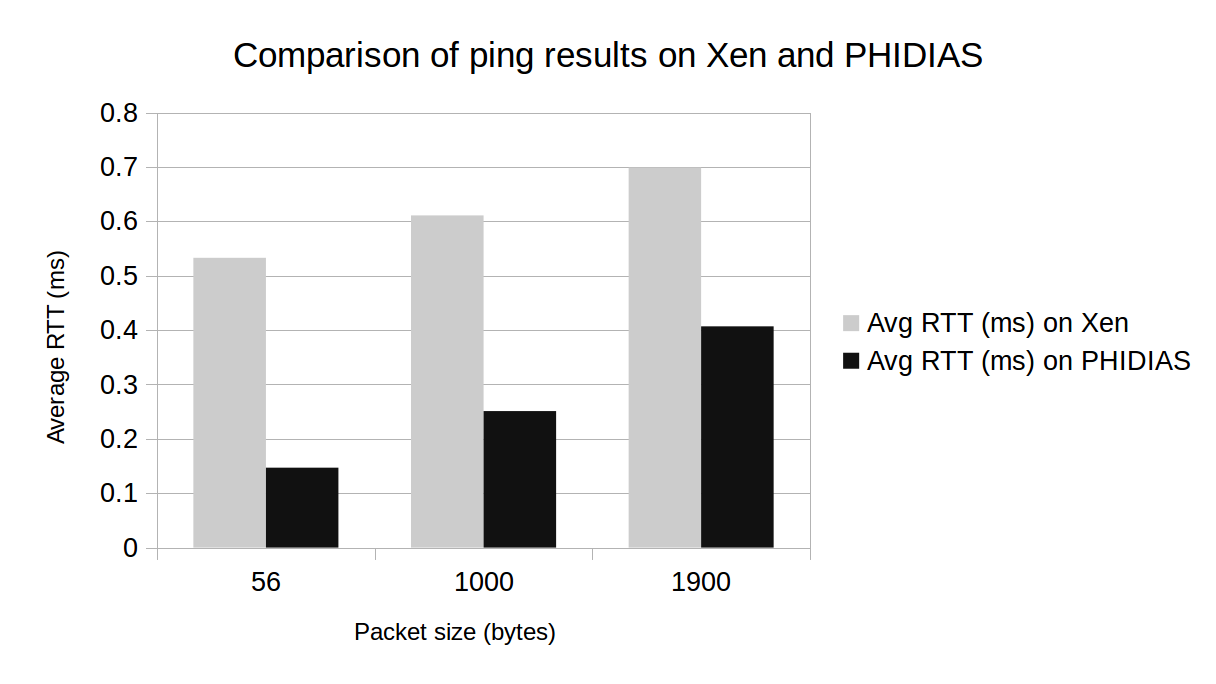
\includegraphics[width=10cm]{ping_rtt}
	\caption{Comparison between round trip latencies of ping packets on PHIDIAS and Xen}
	\label{ping_rtt}
\end{figure}

\begin{figure}[!htbp]
	\centering
	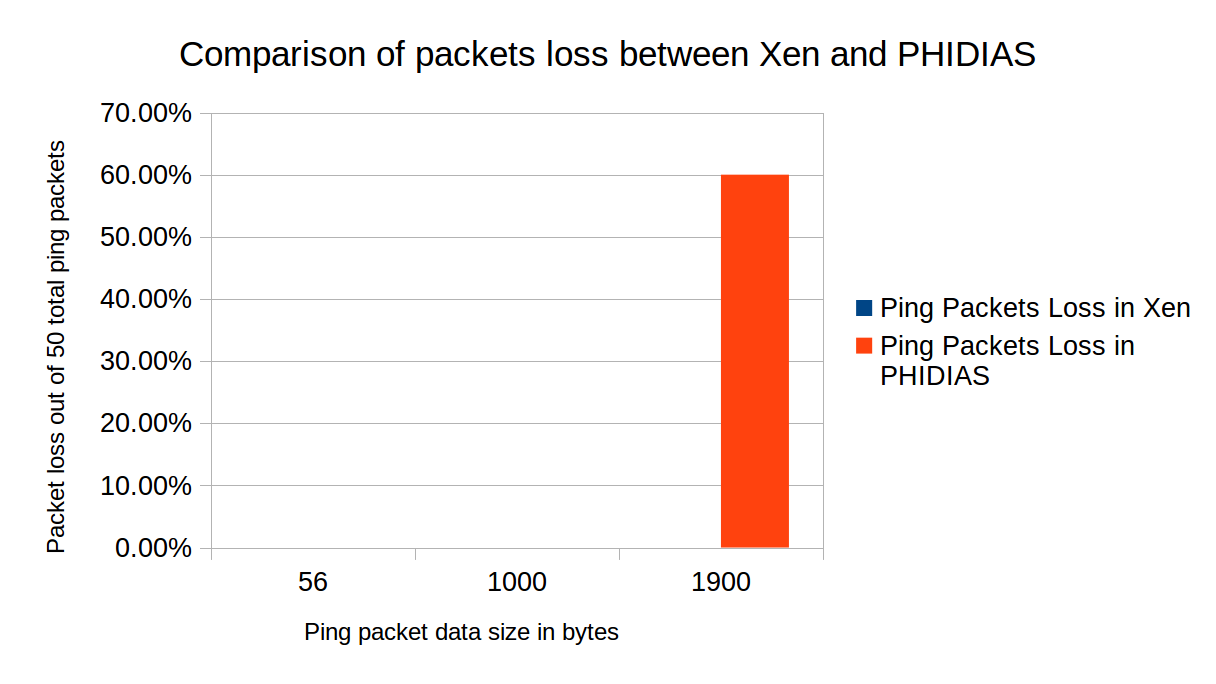
\includegraphics[width=10cm]{ping_loss}
	\caption{Comparison between loss of ping packets on PHIDIAS and Xen}
	\label{ping_loss}
\end{figure}


\section{Network Throughput Test \label{sec:testenvthrough}}
Iperf is the most commonly tool used for measuring throughput. Iperf is based on a client and server model, and can measure the throughput between the two ends in one or both directions using data streams \cite{iperf_wiki}.
\\
\\
For conducting tests, iperf version 2.0.10 (11 Aug 2017) for pthreads \cite{iperf} was used. The tool was cross-compiled for ARM architecture and run in Dom0 and DomU linux guests. Two types were tests were conducted reversing the roles of client and server between Dom0 and DomU guests. Each test was conducted five times in a specific context and then average was calculated for final reading. Default TCP window size of 85.3 KBytes was used for all tests and each test lasted for the default 10.0 sec interval duration.

\subsection{Network Throughput Test results on Xen \label{sec:testthroughxen}}
Table \ref{Iperf_xen} shows the results of two types of iperf tests performed between Dom0 and DomU through virtual network devices on Xen. For the first test, iperf client was run in Dom0 sending data to the iperf server in DomU and for the second test, roles were reversed.

\begin{table}[htbp]
	\caption{Iperf test results on Xen}
	 \centering
	 \resizebox{\textwidth}{!}{
	\begin{tabular}{|l|l|l|l|l|l|}
		\hline
		\textbf{Iperf Client} & \textbf{Iperf Server} & \textbf{TCP  window size on server and client} & \textbf{Interval duration} & \textbf{Transfer Bytes} & \textbf{Bandwidth} \\ \hline
		Dom0 & DomU & 85.3 KBytes (default) & 10.0 sec & 1.582 Gbytes & 1.358 Gbits/sec \\ \hline
		DomU & Dom0 & 85.3 KBytes (default) & 10.0 sec & 1.502 Gbytes & 1.29   Gbits/sec \\ \hline
	\end{tabular}}
	\label{Iperf_xen}
\end{table}

\subsection{Network Throughput Test results on PHIDIAS \label{sec:testthroughphidias}}
Table \ref{Iperf_phidias} shows the results of two types of iperf tests on PHIDIAS with first test making Dom0 as an iperf client and DomU as server and the second test with reversed roles for guests.

\begin{table}[htbp]
	\caption{Iperf test results on PHIDIAS}
	 \centering
	 \resizebox{\textwidth}{!}{
	\begin{tabular}{|l|l|l|l|l|l|}
		\hline
		\textbf{Iperf Client} & \textbf{Iperf Server} & \textbf{TCP  window size on server and client} & \textbf{Interval duration} & \textbf{Transfer Bytes} & \textbf{Bandwidth} \\ \hline
		Dom0 & DomU & 85.3 KBytes (default) & 10.8 sec & 429.6  Kbytes & 328.6 Kbits/s \\ \hline
		DomU & Dom0 & 85.3 KBytes (default) & 10.0 sec & 815.144 Kbytes & 602.8 Kbits/s \\ \hline
	\end{tabular}}
	\label{Iperf_phidias}
\end{table}

\subsection{Analysis of Network Throughput Test results on PHIDIAS \label{sec:testthrougheval}}
Figure \ref{iperf_band} shows the comparison between throughput measurements on XEN and PHIDIAS for both test scenarios.

\begin{figure}[!htbp]
	\centering
	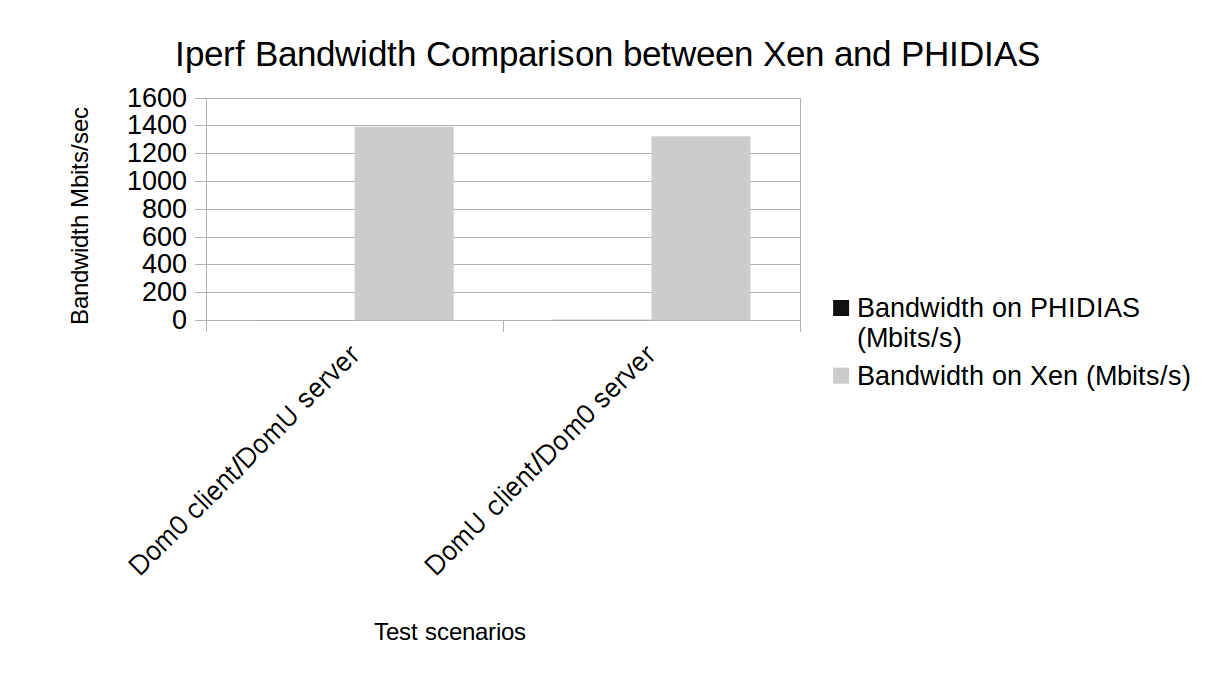
\includegraphics[width=10cm]{iperf_band}
	\caption{Comparison between bandwidth measurements of Iperf on PHIDIAS and Xen}
	\label{iperf_band}
\end{figure}

Figure \ref{iperf_data} shows the comparison between data transferred on XEN and PHIDIAS for the iperf tests on XEN and PHIDIAS.

\begin{figure}[!htbp]
	\centering
	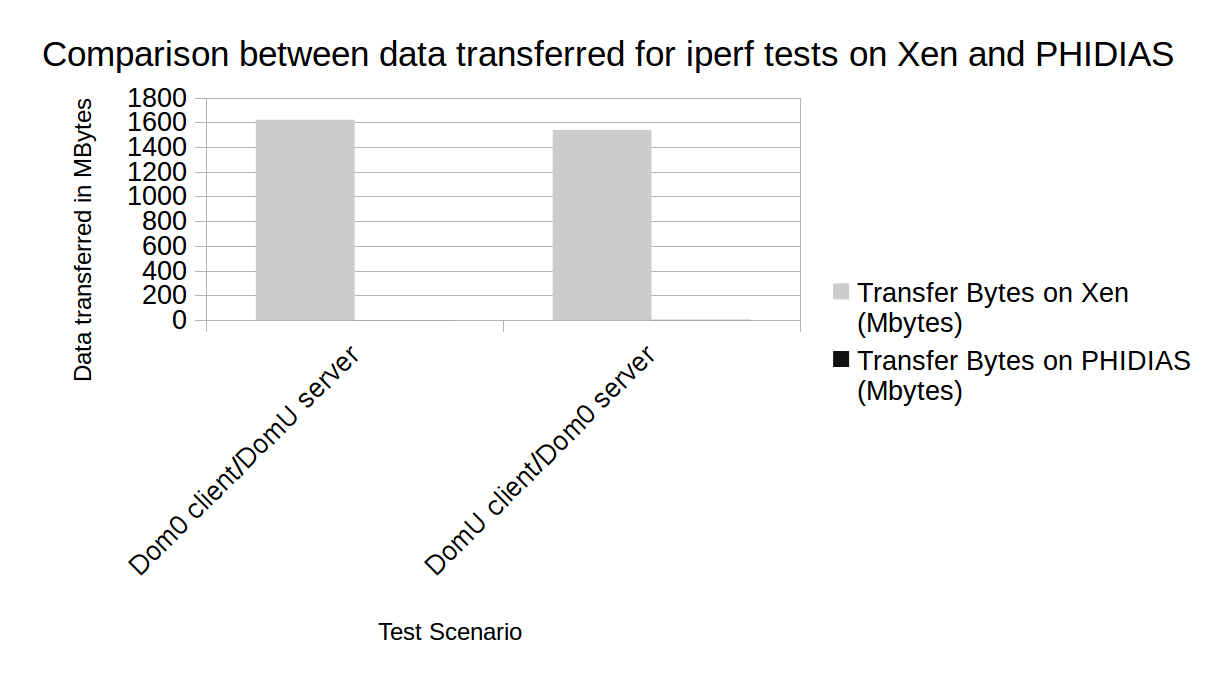
\includegraphics[width=10cm]{iperf_data}
	\caption{Comparison between amount of data transferred for iperf tests on PHIDIAS and Xen}
	\label{iperf_data}
\end{figure}
Figures \ref{iperf_band} and \ref{iperf_data} clearly shows a large difference in throughput measurements between XEN and PHIDIAS. Main reasons for this is same as described in section \ref{sec:testlatencyeval}. Iperf transfers the data depending upon the TCP window size set on both sides which is 85.3 KBytes by default. If the amount of data sent is larger than MTU, fragmentation occurs. From the results, it is obvious that large amount of fragmentation has happened which had caused IP reassembly timeout due to larger time spent in memcpy operations on PHIDIAS.  

